\documentclass[a4paper, 11pt, oneside]{article}

\usepackage[utf8]{inputenc}
\usepackage[T1]{fontenc}
\usepackage[english]{babel}
\usepackage{array}
\usepackage{shortvrb}
\usepackage{listings}
\usepackage[fleqn]{amsmath}
\usepackage{amsfonts}
\usepackage{fullpage}
\usepackage{enumerate}
\usepackage{enumitem}
\usepackage{graphicx}
\usepackage{subfigure}
\usepackage{alltt}
\usepackage{indentfirst}
\usepackage{eurosym}
\usepackage{listings}
\usepackage{titlesec, blindtext, color}
\usepackage{float}
\usepackage[colorlinks, linkcolor=blue]{hyperref}
\usepackage[nameinlink,noabbrev]{cleveref}
\usepackage{caption}
\usepackage{subcaption}

\usepackage{titling}
\renewcommand\maketitlehooka{\null\mbox{}\vfill}
\renewcommand\maketitlehookd{\vfill\null}

\definecolor{mygray}{rgb}{0.5,0.5,0.5}
\definecolor{pink1}{rgb}{0.858, 0.188, 0.478}
\definecolor{sienna}{rgb}{0.53, 0.18, 0.09}
\definecolor{sepia}{rgb}{0.44, 0.26, 0.08}
\definecolor{midnightblue}{rgb}{0.1, 0.1, 0.44}

\renewcommand{\lstlistingname}{Code}

\lstset{
    language=C, % Utilisation du langage C
    commentstyle={\color{MidnightBlue}}, % Couleur des commentaires
    frame=single, % Entoure le code d'un joli cadre
    rulecolor=\color{black}, % Couleur de la ligne qui forme le cadre
    numbers=left, % Ajoute une numérotation des lignes à gauche
    numbersep=5pt, % Distance entre les numérots de lignes et le code
    numberstyle=\tiny\color{mygray}, % Couleur des numéros de lignes
    basicstyle=\tt\footnotesize, 
    tabsize=3, % Largeur des tabulations par défaut
    extendedchars=true, 
    captionpos=b, % sets the caption-position to bottom
    texcl=true, % Commentaires sur une ligne interprétés en Latex
    showstringspaces=false, % Ne montre pas les espace dans les chaines de caractères
    escapeinside={(>}{<)}, % Permet de mettre du latex entre des <( et )>.
    inputencoding=utf8,
    literate=
  {á}{{\'a}}1 {é}{{\'e}}1 {í}{{\'i}}1 {ó}{{\'o}}1 {ú}{{\'u}}1
  {Á}{{\'A}}1 {É}{{\'E}}1 {Í}{{\'I}}1 {Ó}{{\'O}}1 {Ú}{{\'U}}1
  {à}{{\`a}}1 {è}{{\`e}}1 {ì}{{\`i}}1 {ò}{{\`o}}1 {ù}{{\`u}}1
  {À}{{\`A}}1 {È}{{\`E}}1 {Ì}{{\`I}}1 {Ò}{{\`O}}1 {Ù}{{\`U}}1
  {ä}{{\"a}}1 {ë}{{\"e}}1 {ï}{{\"i}}1 {ö}{{\"o}}1 {ü}{{\"u}}1
  {Ä}{{\"A}}1 {Ë}{{\"E}}1 {Ï}{{\"I}}1 {Ö}{{\"O}}1 {Ü}{{\"U}}1
  {â}{{\^a}}1 {ê}{{\^e}}1 {î}{{\^i}}1 {ô}{{\^o}}1 {û}{{\^u}}1
  {Â}{{\^A}}1 {Ê}{{\^E}}1 {Î}{{\^I}}1 {Ô}{{\^O}}1 {Û}{{\^U}}1
  {œ}{{\oe}}1 {Œ}{{\OE}}1 {æ}{{\ae}}1 {Æ}{{\AE}}1 {ß}{{\ss}}1
  {ű}{{\H{u}}}1 {Ű}{{\H{U}}}1 {ő}{{\H{o}}}1 {Ő}{{\H{O}}}1
  {ç}{{\c c}}1 {Ç}{{\c C}}1 {ø}{{\o}}1 {å}{{\r a}}1 {Å}{{\r A}}1
  {€}{{\euro}}1 {£}{{\pounds}}1 {«}{{\guillemotleft}}1
  {»}{{\guillemotright}}1 {ñ}{{\~n}}1 {Ñ}{{\~N}}1 {¿}{{?`}}1
}


\newcommand{\ClassName}{INFO-0027: Programming techniques}
\newcommand{\ProjectName}{Project 1: Performance study}
\newcommand{\AcademicYear}{2020 - 2021}

%%%% Page de garde %%%%

\title{\ClassName\\\vspace*{0.8cm}\ProjectName\vspace{0.8cm}}
\author{Goffart Maxime \\180521 \and Joris Olivier \\ 182113}
\date{\vspace{1cm}Academic year \AcademicYear}

\begin{document}

%%% Page de garde %%%
\begin{titlingpage}
{\let\newpage\relax\maketitle}
\end{titlingpage}

%%%%%%%%%%%%%%%%%%%%%%%%%%%%%%%%%%%%%%%%%%%%%%
\section{Introduction}
\paragraph{}We decided to perform our perfomance study by doing 1000 differents creation of the \texttt{MAGIC} A.D.T. and by measuring the mean time passed in the \texttt{MAGICindex} and \texttt{MAGICreset} functions and the mean amount of allocated memory. 
\paragraph{}We chose to deal with an increasing number of addresses to be able to analyse the differences between the implementation on graphics. The addresses we used to perform our studies were randomly generated 4 bytes addresses. We used the same randomly generated batch of addresses for the two different implementations.

\section{Time perfomance}

\subsection{Mean time passed in the MAGICindex function}

\begin{figure}[H]
  \centering
  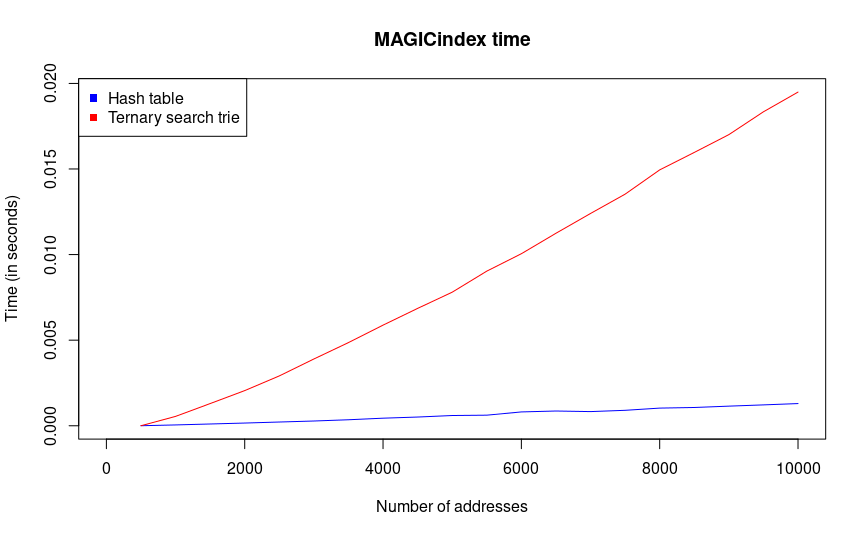
\includegraphics[scale=.6]{plots/index.png}
  \captionof{figure}{Mean total time passed in the MAGICindex function according to the number of addresses of our two implementations.}
\end{figure}

\subsection{Mean time passed in the MAGICreset function}

\begin{figure}[H]
  \centering
  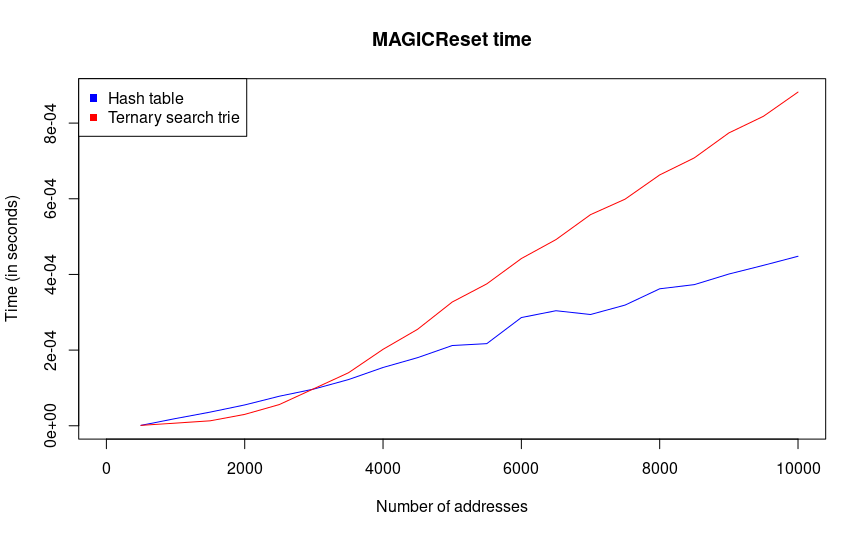
\includegraphics[scale=.6]{plots/reset.png}
  \captionof{figure}{Mean total time passed in the MAGICreset function according to the number of addresses of our two implementations.}
\end{figure}


\subsection{Sum of the two previous mean times}

\begin{figure}[H]
  \centering
  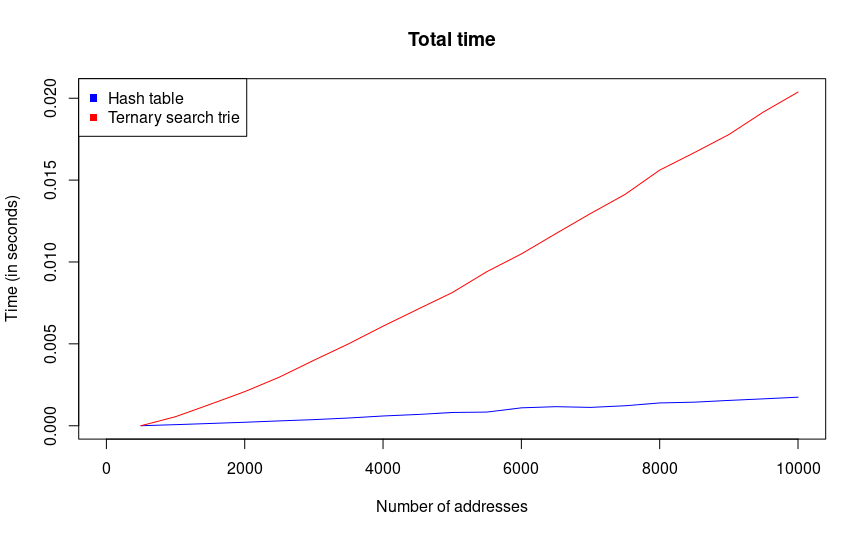
\includegraphics[scale=.6]{plots/general.png}
  \captionof{figure}{Mean total time passed in the A.D.T. functions according to the number of addresses of our two implementations.}
\end{figure}

\section{Memory perfomance}

\begin{figure}[H]
  \centering
  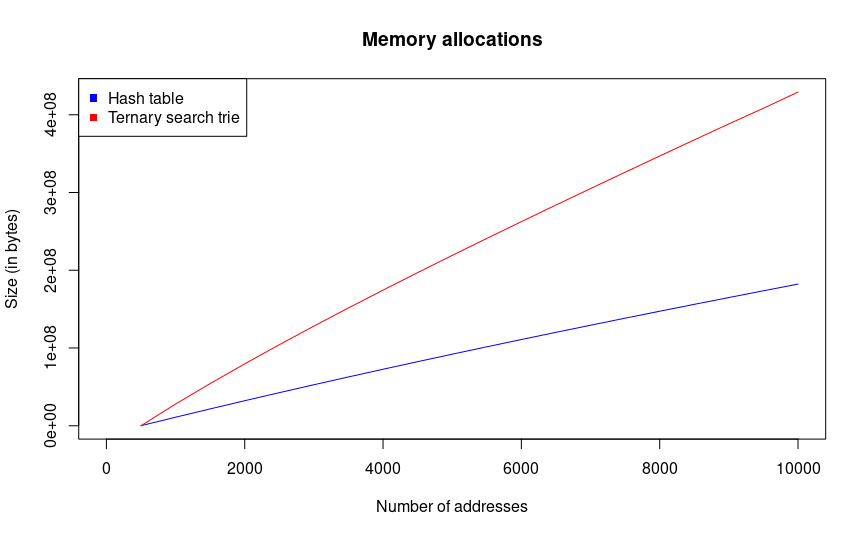
\includegraphics[scale=.6]{plots/mem.png}
  \captionof{figure}{Mean amount of memory allocated according to to the number of addresses of our two implementations.}
\end{figure}

\section{Conclusion}
\paragraph{}In conclusion, we observe that our first implementation (hash table) has better perfomances than our second one (ternary search trie) in terms of time and memory.

\end{document}
